
\chapter{Combinatorics}

\section{Fibonacci pets}

In \autoref{combinatorics:fibonacci:pets} we report a pretty nice 
picture showing Fibonacci numbers characterized by pets population
evolution.

Assume to look at the table as if it is a lower triangular infinite
matrix, and denote with $w_{n+1,k+1}$ the number of white \emph{child}
pets at row $n+1$ and column $k+1$; similarly, denote with 
$b_{n+1,k+1}$ the number of brown \emph{parent} pets at row $n+1$ and column $k+1$.

We can derive the following relation over $w_{n+1,k+1}$:
\begin{displaymath}
    w_{n+1,k+1} = b_{n,k}
\end{displaymath}
and the following one over $b_{n+1,k+1}$:
\begin{displaymath}
    b_{n+1,k+1} = b_{n,k+1} + w_{n,k+1}
\end{displaymath}
which, by mutual definition, can be rewritten as:
\begin{displaymath}
    b_{n+1,k+1} = b_{n,k+1} + b_{n-1,k}
\end{displaymath}
so, summing white and brown pair of pets at the same entry we have:
\begin{displaymath}
    b_{n+1,k+1}+w_{n+1,k+1} = b_{n,k+1} + b_{n-1,k} + b_{n,k}
\end{displaymath}
such relation characterize the matrix using \emph{brown} pairs of pets only,
namely \emph{parent} pets.


\begin{figure}[p]

    \noindent\makebox[\textwidth]{
        \centering
        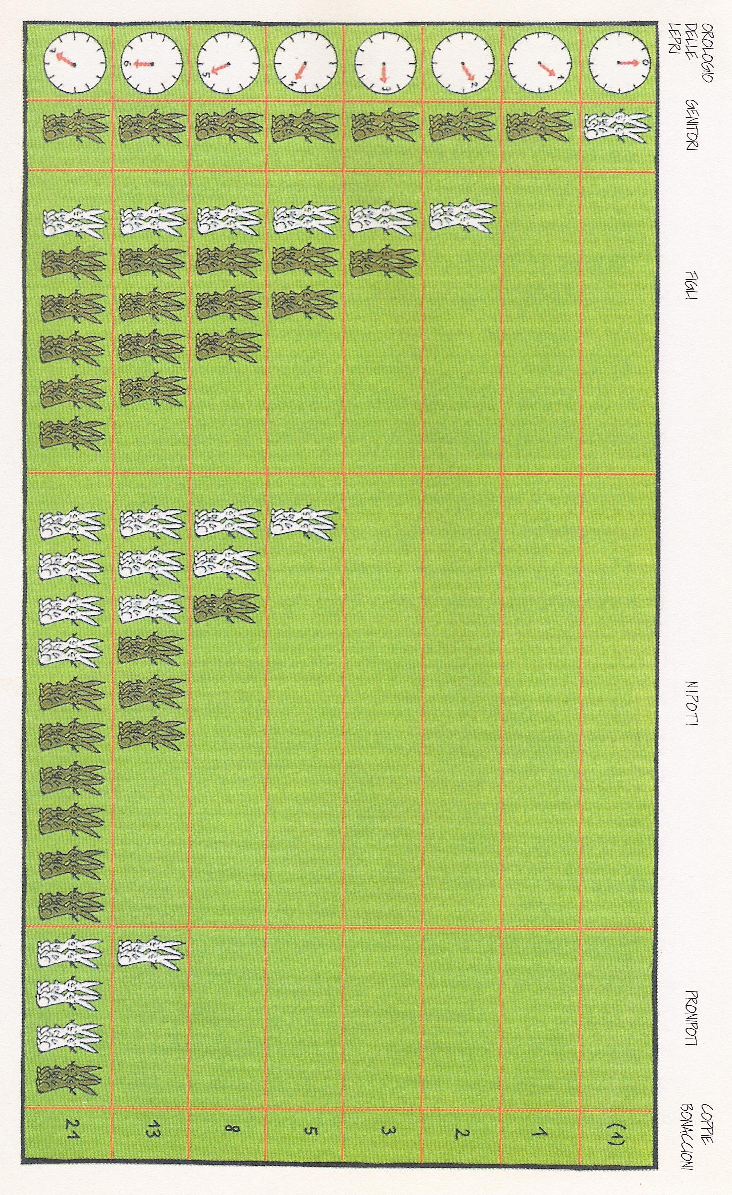
\includegraphics[width=0.8\textwidth, keepaspectratio=true, angle=90]{gfx/combinatorics/fibonacci-pets.pdf}

        % using *angle* property to rotate it is difficult to properly align it
        % in order to have a "real" matrix representation.
        %\includegraphics[width=20cm, height=20cm, keepaspectratio=true]{../sympy/pascal/pascal-inverse-handle-negatives-centered-colouring-127-rows-mod2-partitioning-triangle.pdf}
    }

    % this 'particular' line is necessary to use `displaymath' environment
    % into the caption environment, togheter with the inclusion of 
    % `caption' package. See here for more explanation:
    % http://stackoverflow.com/questions/2716227/adding-an-equation-or-formula-to-a-figure-caption-in-latex
    \captionsetup{singlelinecheck=off}
    \caption[.]{Fibonacci pets}
    \label{combinatorics:fibonacci:pets}

\end{figure}
